\documentclass[a4paper,12pt]{article} % добавить leqno в [] для нумерации слева
\usepackage[a4paper,top=1.3cm,bottom=2cm,left=1.5cm,right=1.5cm,marginparwidth=0.75cm]{geometry}
%%% Работа с русским языком
\usepackage{cmap}					% поиск в PDF
\usepackage{mathtext} 				% русские буквы в фомулах
\usepackage[T2A]{fontenc}			% кодировка
\usepackage[utf8]{inputenc}			% кодировка исходного текста
\usepackage[english,russian]{babel}	% локализация и переносы
\usepackage{siunitx}

\usepackage{graphicx}

\usepackage{wrapfig}
\usepackage{tabularx}

\usepackage{hyperref}
\usepackage[rgb]{xcolor}
\hypersetup{
colorlinks=true,urlcolor=blue
}

%%% Дополнительная работа с математикой
\usepackage{amsmath,amsfonts,amssymb,amsthm,mathtools} % AMS
\usepackage{icomma} % "Умная" запятая: $0,2$ --- число, $0, 2$ --- перечисление

%% Номера формул
\mathtoolsset{showonlyrefs=true} % Показывать номера только у тех формул, на которые есть \eqref{} в тексте.

%% Шрифты
\usepackage{euscript}	 % Шрифт Евклид
\usepackage{mathrsfs} % Красивый матшрифт

%% Свои команды
\DeclareMathOperator{\sgn}{\mathop{sgn}}

%% Перенос знаков в формулах (по Львовскому)
\newcommand*{\hm}[1]{#1\nobreak\discretionary{}
{\hbox{$\mathsurround=0pt #1$}}{}}

%%% Заголовок
\author{Макаров Лев Евгеньевич}
\title{Лабораторная работа №1.2.1

Определение скорости полета пули при помощи баллистического маятника
}
\date{\today}

\begin{document}

\begin{titlepage}
	\begin{center}
		{\large МОСКОВСКИЙ ФИЗИКО-ТЕХНИЧЕСКИЙ ИНСТИТУТ (НАЦИОНАЛЬНЫЙ ИССЛЕДОВАТЕЛЬСКИЙ УНИВЕРСИТЕТ)}
	\end{center}
	\begin{center}
		{\large Физтех-школа фотоники, электроники и молекулярной физики}
	\end{center}
	
	
	\vspace{4.5cm}
	{\huge
		\begin{center}
			{\bf Отчёт о выполнении лабораторной работы 1.2.1}\\
			Определение скорости полета пули при помощи баллистического маятника
		\end{center}
	}
	\vspace{2cm}
	\begin{flushright}
		{\LARGE Автор:\\ Макаров Лев Евгеньевич \\
			\vspace{0.2cm}
			Б04-306}
	\end{flushright}
	\vspace{8cm}
	\begin{center}
		Долгопрудный 2023
	\end{center}
\end{titlepage}

\section{Введение}

\textbf{Цель работы:} определить скорость полета пули, применяя законы сохранения и используя баллистические маятники.
\medskip

\textbf{В работе используются:} 
\begin{itemize}
    \item духовое ружье на штативе
    \item осветитель
    \item оптическая система для измерения отклонений маятника
    \item измерительная линейка
    \item пули
    \item электронные весы B1203 (для измерения пулек)
    \item электронные весы EK-6100i (для измерения массы грузов)
    \item два баллистических маятника с разными конструкциями
\end{itemize}
\medskip

В работе используются следующие методы измерения скорости:
\begin{enumerate}
	\item Метод баллистического маятника, совершающего поступательное движение;
	\item Метод крутильного баллистического маятника
\end{enumerate}

\section{Теоретические сведения}

\label{p2}


\subsection{Метод баллистического маятника, совершающего поступательное движение}
\label{p2-1}
\begin{figure}[h]
    \begin{center}$
        \begin{array}{cc}
            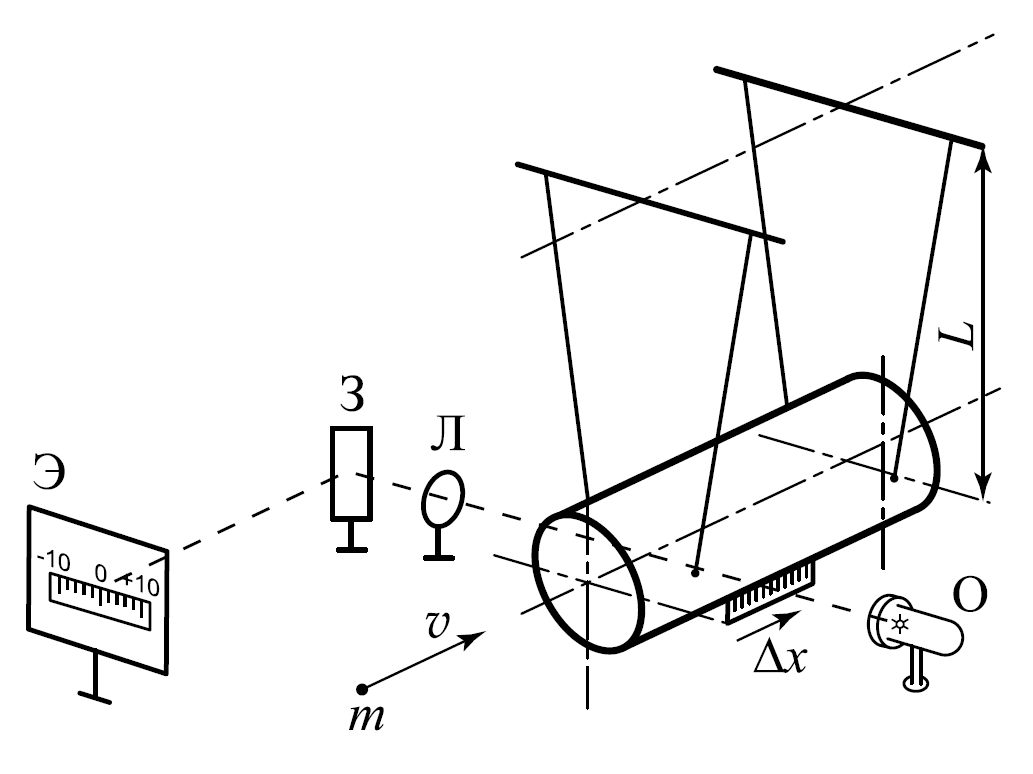
\includegraphics[width=0.45\textwidth]{ustan1-1.png}&
            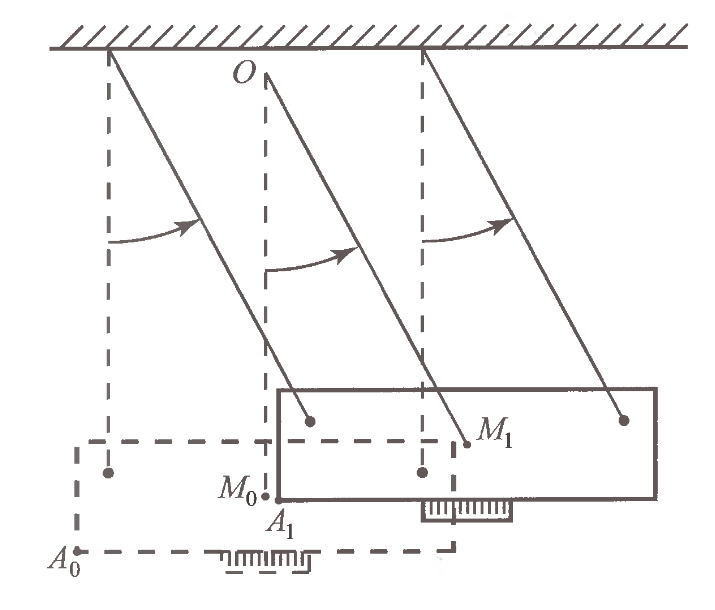
\includegraphics[width=0.45\textwidth]{ustan1-2.png}\\
            % \text{рис. 1: схема установки} & \text{рис. 2: поведение баллистического маятника}\\
            % &\text{при попадании в него пули.}
        \end{array}$
    \end{center}
    \caption{Схема установки и её поведения при попадании в неё пули}
    \label{fig:ustan1}
\end{figure}

В этой части используется установка, изображенная на \textit{рис.  \ref{fig:ustan1}}. Закон сохранения импульса при соударении пули с цилиндром имеет вид:
\begin{equation}\label{1form}
mu = (M + m)V
\end{equation}

Здесь $m$ -- масса пули, $M$ -- масса цилиндра, $u$ -- скорость пули перед ударом, $V$ -- скорость цилиндра и пули после неупругого соударения. Так как масса маятника сильно больше массы пули, то из \eqref{1form} получаем:

\begin{equation}\label{2form}
u = \frac{M}{m}V
\end{equation}

По закону сохранения энергии высота $h$ подъёма маятника над его начальным положением связана с $V$ следующим образом:

\begin{equation}\label{3form}
V^2 = 2gh
\end{equation}

Высота подъёма маятника выражается через угол $\phi$ отклонения маятника от вертикали:

\begin{equation}\label{4form}
h = L(1 - \cos\varphi) = 2L \sin^2{\frac{\varphi}{2}} \text{, где } \varphi \approx \frac{\Delta x}{L}
\end{equation}

Из \eqref{2form}, \eqref{3form}, \eqref{4form} получаем следует окончательная формула \eqref{5form} для определения скорости пули:

\begin{equation}\label{5form}
u = \frac{M}{m} \sqrt{\frac{g}{L}} \Delta x
\end{equation}

Измерение отклонения маятника $\Delta x$ производится с помощью оптической системы, изображённой на \textit{рис.  \ref{fig:ustan1}}.


\subsection{Метод крутильного баллистического маятника}
\label{p2-2}

В этом методе используется установка, изображенная на \textit{рис.  \ref{fig:ustan2}}.
\begin{figure}[h!]
    \begin{center}$
        \begin{array}{c}
            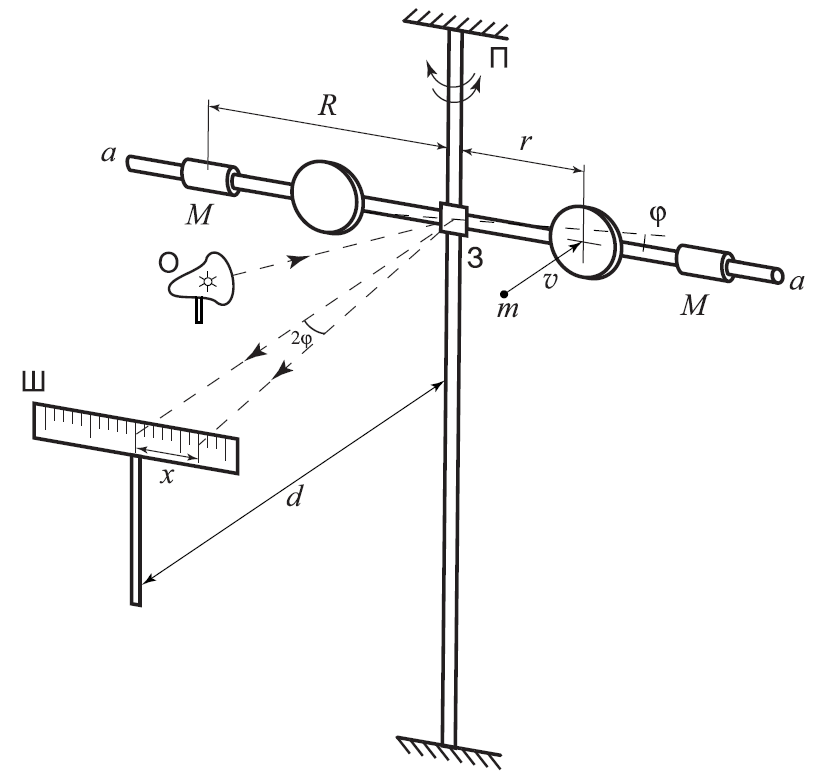
\includegraphics[width=0.60\textwidth]{ustan2.png}\\
        \end{array}$
    \end{center}
    \caption{Крутильный баллистический маятник.}
    \label{fig:ustan2}
\end{figure}

Пуля массой $m$ попадает в мишень, укреплённую на стержне $aa$ который вместе с грузами $M$ и проволокой $П$ образуют крутильный маятник. Для определения скорости $u$ полёта пули прямо перед ударом воспользуемся законом сохранения момента импульса:

\begin{equation}\label{6form}
mur = I\Omega
\end{equation}

Здесь $r$ -- расстояние от линии полёта пули до оси вращения маятника, $I$ -- момент инерции маятника, $\Omega$ -- его угловая скорость непосредственно после удара. Закон сохранения энергии при колебаниях маятника записываем следующим образом:

\begin{equation}\label{7form}
k \frac{\varphi^2}{2} = I \frac{\Omega^2}{2}
\end{equation}

Здесь $k$ -- модуль кручения проволоки $П$, $\varphi$ -- максимальный уголповорота маятника. Из \eqref{6form} и \eqref{7form} получаем:

\begin{equation}\label{8form}
u = \varphi \frac{\sqrt{kI}}{mr}
\end{equation}

$\varphi$ в данных опытах всегда мал и находится по смещению $x$ точки лазера на измерительной шкале:

\begin{equation}\label{9form}
\varphi \approx \frac{x}{d}
\end{equation}

Здесь $d$ -- расстояние от шкалы $Ш$ до оси вращения маятника.

Произведение $kI$, входящее в формулу \eqref{8form}, можно найти по измерениям периодов колебаний маятника с грузами $M$ и без них. В первом случае:

\begin{equation}\label{10form}
T_1 = 2\pi \sqrt{\frac{I}{k}}
\end{equation}

Во втором случае:

\begin{equation}\label{11form}
T_2 = 2\pi \sqrt{\frac{I - 2MR^2}{k}}
\end{equation}

Из формул \eqref{10form} и \eqref{11form} следует:

\begin{equation}\label{12form}
\sqrt{kI} = \frac{4\pi MR^2 T_1}{T_1^2 - T_2^2}
\end{equation}

Здесь $R$ -- расстояние от центров масс грузов $M$ до проволоки.

\section{Оборудование и экспериментальные погрешности}

\textbf{электронные весы B1203:} $\Delta_m = \pm 0,0001$ г \\
\textbf{электронные весы EK-6100i:} $\Delta_M = \pm 5$ г \\
\textbf{Изсерительная линейка:} $\Delta = \pm 0,1$ см \\

\textbf{Измеренные параметры баллистических маятников:}

\begin{table}[htbp]
  \begin{minipage}[t]{0.5\textwidth}
    \centering
        \begin{tabular}{|c|c|}
          \hline
          Характеристика & Значение \\ \hline
          M, г & $2925,0 \pm 5,0$ \\ \hline
          L, мм & $2217,5 \pm 10,0$ \\ \hline
        \end{tabular}
    \caption{\textit{Параметры маятника на \textit{рис.  \ref{fig:ustan1}}}}
  \end{minipage}%
  \begin{minipage}[t]{0.5\textwidth}
    \centering
        \begin{tabular}{|c|c|}
          \hline
          Характеристика & Значение \\ \hline
          M, г & $732,3 \pm 5,0$ \\ \hline
          d, см & $130,0 \pm 0,1$ \\ \hline
          r, см & $21,4 \pm 0,1$ \\ \hline
          R, см & $33,6 \pm 0,1$ \\ \hline
        \end{tabular}
    \caption{\textit{Параметры маятника на \textit{рис.  \ref{fig:ustan2}}}}
  \end{minipage}
\end{table}

\pagebreak

\section{Результаты измерений и обработка данных}

Измерения масс десяти пулек, используемых для выстрелов, электронными весами B1203 представлены в \textit{Таблице  \ref{tab:tab1}} (номера пулек соответствуют номерам последующих выстрелов).

\begin{table}[h]
    \begin{tabular}{|l|l|l|l|l|l|l|l|l|l|l|}
        \hline
        N (номер пульки) & 1 & 2 & 3 & 4 & 5 & 6 & 7 & 8 & 9 & 10 \\
        \hline
        m\text{, г} & 0.508 & 0.510 & 0.511 & 0.497 & 0.491 & 0.507 & 0.502 & 0.504 & 0.502 & 0.504 \\
        \hline
    \end{tabular}
    \caption{\textit{Измерение масс пулек электронными весами B1203}}
    \label{tab:tab1}
\end{table}


\subsection{Метод баллистического маятника, совершающего поступательное движение}


Измерения аксимальной амплитуды можно использовать только если после десяти колебаний баллистического маятника амплитуда уменьшилась не более чем вдвое. Результаты этих измерений представлены в \textit{Таблице \ref{tab:tab-amp}}:

\begin{table}[!ht]
    \centering
    \begin{tabular}{|c|c|c|c|c|c|}
    \hline
        N (номер выстрела) & 1 & 2 & 3 & 4 & 5 \\ \hline
        $\Delta x$, мм & 12,5 & 12,5 & 12,0 & 12,0 & 12,0 \\ \hline
    \end{tabular}
    \caption{\textit{Измерение скорости пули}}
    \label{tab:tab-amp}
\end{table}

Среднее значение амплитуды отклонения $ \overline{\Delta x} = \frac{\Delta x_i}{N} = 12,20 \text{ мм}$.\\

Случайная погрешность измерения $ \sigma_{\overline{\Delta x}} = \sqrt{\frac{1}{N  (N-1)}\sum(\Delta x_i-\overline{\Delta x})^2} \approx 0,12 \text{ мм}$.\\

С учётом инструментальной погрешности $ \Delta_\text{шкалы} = 0,20$ мм погрешность амплитуды отклонения может быть вычислена как $ \sigma_{\Delta x} = \sqrt{\sigma^2_{\overline{\Delta x}} + \Delta^2_{\text{шкалы}}} \approx 0,23 \text{ мм}$. \\


Погрешность измерения скорости пули можно рассчитать по формуле:

\begin{equation}
\sigma_u = u \sqrt{\left( \frac{\sigma_M}{M} \right) ^2 + \left( \frac{\sigma_m}{m} \right) ^2 + \left( \frac{\sigma_L}{L} \right) ^2 + \left( \frac{\sigma_{\Delta x}}{\Delta x} \right) ^2}.
\label{13form}
\end{equation}

Вычисленные по формуле \eqref{5form} значения скорости пулек представлены в \textit{Таблице  \ref{tab:tab2}}

\begin{table}[!ht]
    \centering
    \begin{tabular}{|c|c|c|c|c|c|}
    \hline
        N (номер выстрела) & 1 & 2 & 3 & 4 & 5 \\ \hline
        $u$, м/с & 151,3 & 150,7 & 144,4 & 148,5 & 150,3 \\ \hline
        $\sigma_u$, м/с & 2,5 & 2,5 & 2,5 & 2,6 & 2,6 \\ \hline
        $\varepsilon_u$, \% & 1,7 & 1,7 & 1,7 & 1,7 & 1,7 \\ \hline
    \end{tabular}
    \caption{\textit{Измерение скорости пули}}
    \label{tab:tab2}
\end{table}

Среднее значение скорости: $\overline{u} = \left( 149,0 \pm 2,5 \right) \text{ м/с} \left( \varepsilon_\rho = 1,7 \% \right)$\\

\subsection{Метод крутильного баллистического маятника}

С помощью секундамера измерим периоды $T_1 = \left( 6,6 \pm 0,1 \right) \text{ с}$ и $T_2 = \left( 4,9 \pm 0,1 \right) \text{ с}$ как средние значения десяти измерений. По формуле \eqref{12form} вычислим $\sqrt{kI} = 0,350 \text{ м}^2 \text{ кг}/\text{с}$. Погрешность $\sigma_{\sqrt{kI}}$ вычисляется по формуле:

\begin{equation}
    \sigma_{\sqrt{kI}} = \sqrt{kI} \sqrt{ \left( \frac{\sigma_M}{M} \right)^2 + \left( \frac{\sigma_R}{R} \right)^2 + \left( \frac{\sigma_{T_1}}{T_1} \right)^2 + \left( \frac{\sigma_{T_2}}{T_2} \right)^2} = 0,009 \text{ м}^2 \text{ кг}/\text{с}
\end{equation}

Измерим значения $x$ (использовать полученные значения можно только если после десяти колебаний баллистического маятника значение амплитуды уменьшилось не более чем вдвое) с погрешностью $\sigma_x = 0,1 \text{ см}$, по которым вычислим значения углов максимального поворота $\varphi$ по формуле \eqref{9form}, а погрешность угла $\varphi$ вычислим по формуле:

\begin{equation}
    \sigma_\varphi = \varphi \sqrt{ \left( \frac{\sigma_x}{x} \right)^2 + \left( \frac{\sigma_d}{d} \right)^2}
\end{equation}

Результаты измерений $x$, полученные значения $\varphi$ и значения погрешностей $\sigma_\varphi$ представлены в \textit{Таблице \ref{tab:tab-phi}}

\begin{table}[!ht]
    \centering
    \begin{tabular}{|c|c|c|c|c|c|}
    \hline
        N (номер выстрела) & 6 & 7 & 8 & 9 & 10 \\ \hline
        $x$, см & 4,0 & 4,0 & 4,1 & 3,5 & 3,8 \\ \hline
        $\varphi$, рад. & 0,0308 & 0,0308 & 0,0315 & 0,0269 & 0,0292 \\ \hline
        $\sigma_\varphi$, рад. & 0,0008 & 0,0008 & 0,0008 & 0,0008 & 0,0008 \\ \hline
    \end{tabular}
    \caption{\textit{Значения углов $\varphi$}}
    \label{tab:tab-phi}
\end{table}

Используя значение $\sigma_{\sqrt{kI}}$ вычислим значение скорости $u$ для пулек с номерами $N$. А погрешность $\sigma_u$ вычислим по формуле:

\begin{equation}
    \sigma_u = u \sqrt{ \left( \frac{\sigma_{\sqrt{kI}}}{\sqrt{kI}} \right)^2 + \left( \frac{\sigma_m}{m} \right)^2 + \left( \frac{\sigma_r}{r} \right)^2 + \left( \frac{\sigma_\varphi}{\varphi} \right)^2}
\end{equation}

Вычисленные по формуле \eqref{8form} значения скорости пулек представлены в \textit{Таблице  \ref{tab:tab3}}

\begin{table}[!ht]
    \centering
    \begin{tabular}{|c|c|c|c|c|c|}
    \hline
        N (номер выстрела) & 6 & 7 & 8 & 9 & 10 \\ \hline
        $u$, м/с & 99,6 & 100,5 & 102,6 & 88,0 & 95,1 \\ \hline
        $\sigma_u$, м/с & 3,7 & 3,7 & 3,7 & 3,5 & 3,6 \\ \hline
        $\varepsilon_u$, \% & 1,7 & 1,7 & 1,7 & 1,7 & 1,7 \\ \hline
    \end{tabular}
    \caption{\textit{Измерение скорости пули}}
    \label{tab:tab3}
\end{table}

Среднее значение скорости: $\overline{u} = \left( 97,2 \pm 3,6 \right) \text{ м/с} \left( \varepsilon_u = 3,7 \% \right)$\\


\section{Обсуждение результатов и выводы}

Были измерены значения скоростей пуль двумя методами, описанными в пункте \ref{p2}, однако сравнить результаты в полной мере невозможно, так как были использованы разные духовые ружья. Относительная погрешность измерения методом из пункта \ref{p2-1} $\varepsilon_{u_1} = 1,7 \%$, а из пункта \ref{p2-2} $\varepsilon_{u_2} = 3,7 \%$. Измерение скорости пули вторым методом в два раза менее точное, чем измерение первым методом. Это связано с тем, что во втором методе большее количество величин вносят свой вклад в конечную погрешность измерения.

\end{document}